\documentclass[12pt,a4paper]{article}

% ─── Encoding ───
\usepackage[utf8]{inputenc}
\usepackage[T1]{fontenc}

% ─── Page layout ───
\usepackage[margin=2.5cm]{geometry}

% ─── Math ───
\usepackage{amsmath,amssymb,amsthm,mathtools}

% ─── Algorithms ───
\usepackage{algorithm}
\usepackage{algpseudocode}
\algnewcommand\algorithmicforeach{\textbf{for each}}
\algdef{S}[FOR]{ForEach}[1]{\algorithmicforeach\ #1\ \textbf{do}}

% ─── TikZ ───
\usepackage{tikz}
\usetikzlibrary{shapes.geometric,arrows.meta,positioning,fit,
                backgrounds,calc,decorations.pathreplacing,matrix,chains}

% ─── Tables ───
\usepackage{booktabs}
\usepackage{tabularx}
\usepackage{multirow}
\usepackage{array}
\usepackage{float}
\usepackage{longtable}

% ─── Code listings ───
\usepackage{listings}
\usepackage{xcolor}

% ─── Misc ───
\usepackage{caption}
\usepackage{subcaption}
\usepackage{enumitem}
\usepackage{hyperref}
\hypersetup{colorlinks=true,linkcolor=blue!70!black,pdftitle={encoders.py Annotated Reference}}

% ─── Headers ───
\usepackage{fancyhdr}
\pagestyle{fancy}
\fancyhf{}
\lhead{\footnotesize MIVA-KNIGHT \texttt{encoders.py} — Annotated Technical Reference}
\rhead{\footnotesize IT 581 Project}
\cfoot{\thepage}

% ─── Theorem environments ───
\theoremstyle{definition}
\newtheorem{theorem}{Theorem}[section]
\newtheorem{lemma}[theorem]{Lemma}
\newtheorem{definition}[theorem]{Definition}
\newtheorem{axiom}[theorem]{Axiom}
\newtheorem{proposition}[theorem]{Proposition}
\newtheorem{corollary}[theorem]{Corollary}
\theoremstyle{remark}
\newtheorem{remark}[theorem]{Remark}

% ─── Colours ───
\definecolor{cBlue}{RGB}{220,230,245}
\definecolor{cGreen}{RGB}{210,240,210}
\definecolor{cOrange}{RGB}{255,235,215}
\definecolor{cGray}{RGB}{230,230,230}
\definecolor{cPurple}{RGB}{235,220,245}
\definecolor{cTeal}{RGB}{200,235,235}
\definecolor{cYellow}{RGB}{255,248,200}
\definecolor{cDark}{RGB}{40,60,100}
\definecolor{cRed}{RGB}{245,220,220}
\definecolor{cMed}{RGB}{200,240,230}
\definecolor{cWhisper}{RGB}{255,240,210}

% ─── Code style ───
\lstset{
  language=Python,
  basicstyle=\ttfamily\footnotesize,
  keywordstyle=\color{blue!70!black}\bfseries,
  commentstyle=\color{green!50!black}\itshape,
  stringstyle=\color{orange!70!black},
  numberstyle=\tiny\color{gray},
  frame=single, rulecolor=\color{gray!40},
  numbers=left, breaklines=true,
  tabsize=4, showstringspaces=false,
  morekeywords={dataclass,abstractmethod,ABC,Optional,List,torch,nn,F}
}

% ─── TikZ styles ───
\tikzset{
  basebox/.style={rectangle,rounded corners=4pt,draw=black!60,
                  align=center,font=\footnotesize},
  bluenode/.style={basebox,fill=cBlue,minimum width=3cm,minimum height=0.85cm},
  greennode/.style={basebox,fill=cGreen,minimum width=3cm,minimum height=0.85cm,thick},
  orangenode/.style={basebox,fill=cOrange,minimum width=3cm,minimum height=0.85cm},
  graynode/.style={basebox,fill=cGray,minimum width=3cm,minimum height=0.85cm},
  purplenode/.style={basebox,fill=cPurple,minimum width=3cm,minimum height=0.85cm},
  tealnode/.style={basebox,fill=cTeal,minimum width=3cm,minimum height=0.85cm},
  mednode/.style={basebox,fill=cMed,minimum width=3cm,minimum height=0.85cm,thick},
  whisnode/.style={basebox,fill=cWhisper,minimum width=3cm,minimum height=0.85cm},
  warnnode/.style={basebox,fill=cRed,minimum width=3cm,minimum height=0.85cm},
  frozennode/.style={basebox,fill=cGray,minimum width=3.2cm,minimum height=0.85cm,
                     draw=red!60,dashed,thick},
  trainnode/.style={basebox,fill=cBlue,minimum width=3.2cm,minimum height=0.85cm,
                    draw=green!60,thick},
  outnode/.style={basebox,fill=cPurple,minimum width=3.2cm,minimum height=0.85cm},
  decnode/.style={diamond,draw=black!70,fill=cYellow,aspect=2.8,
                  align=center,font=\scriptsize},
  arr/.style={->,>=Stealth,thick,color=black!70},
  thkarr/.style={->,>=Stealth,very thick,color=cDark},
  dasharr/.style={->,>=Stealth,dashed,thick,color=gray!60},
  redarr/.style={->,>=Stealth,thick,color=red!60!black},
  grnarr/.style={->,>=Stealth,thick,color=green!50!black},
  bluarr/.style={->,>=Stealth,thick,color=blue!60!black}
}

\renewcommand{\algorithmicrequire}{\textbf{Input:}}
\renewcommand{\algorithmicensure}{\textbf{Output:}}

%───────────────────────────────────────────────────────────
\begin{document}

% ══════════════════════════════════════════════════
%  TITLE PAGE
% ══════════════════════════════════════════════════
\begin{titlepage}
\centering\vspace*{1.5cm}
{\Huge\bfseries\color{cDark} MIVA-KNIGHT}\\[0.4cm]
{\Large\bfseries \texttt{encoders.py}}\\[0.3cm]
{\large Annotated Mathematical \& Algorithmic Reference}\\[1.0cm]

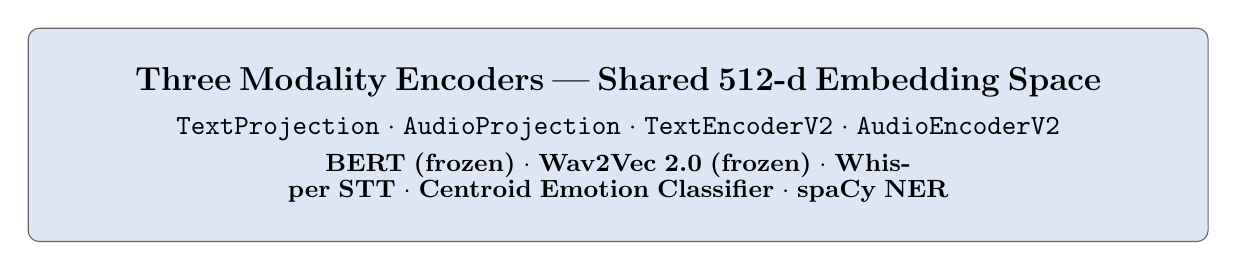
\begin{tikzpicture}
  \node[basebox,fill=cBlue,text width=14cm,inner sep=14pt]{
    \large\bfseries Three Modality Encoders — Shared 512-d Embedding Space\\[4pt]
    \normalsize
    \texttt{TextProjection} $\cdot$ \texttt{AudioProjection} $\cdot$
    \texttt{TextEncoderV2} $\cdot$ \texttt{AudioEncoderV2}\\[4pt]
    \small BERT (frozen) $\cdot$ Wav2Vec 2.0 (frozen) $\cdot$ Whisper STT $\cdot$
    Centroid Emotion Classifier $\cdot$ spaCy NER
  };
\end{tikzpicture}

\vspace{1cm}
{\large\bfseries IT 581 Project}\\[0.3cm]
{\large Oluwakayode Soyinka}\\[0.3cm]
{\normalsize MIVA-KNIGHT: Multimodal Intelligent Voice Assistant — Knight}\\[0.8cm]

\begin{tabular}{ll}
\toprule
\textbf{File}           & \texttt{encoders.py} \\
\textbf{Role}           & Runtime encoder interfaces for text and audio modalities \\
\textbf{Sections}       & Imports, TextProjection, AudioProjection, \_load\_checkpoint, \\
                        & DataContracts, ABCs, TextEncoderV2, AudioEncoderV2,
                          build\_emotion\_centroids \\
\textbf{Backbones}      & BERT-base-uncased (768d, frozen), Wav2Vec 2.0-base (768d, frozen) \\
\textbf{Shared space}   & $\mathbb{S}^{511} \subset \mathbb{R}^{512}$ (unit hypersphere) \\
\textbf{Emotion model}  & RAVDESS 8-class centroid nearest-neighbour classifier \\
\bottomrule
\end{tabular}

\vfill
{\small\color{gray}Each code section below is preceded by formal mathematical
definitions, algorithms, theorems, lemmas, and TikZ flowcharts.
Both technical derivations and plain-language analogies are provided.}
\end{titlepage}

\tableofcontents
\newpage

% ══════════════════════════════════════════════════
\section{Module Overview}
% ══════════════════════════════════════════════════

\subsection{Purpose and Big Picture}

\texttt{encoders.py} provides the \textbf{three modality encoder interfaces}
that map raw inputs into the shared 512-dimensional embedding space
$\mathcal{E} \subset \mathbb{R}^{512}$:

\begin{table}[H]
\centering
\caption{Encoder summary table}
\begin{tabularx}{\textwidth}{lXXX}
\toprule
Encoder & Input & Backbone (frozen) & Head (trained) \\
\midrule
\texttt{TextProjection}         & $\mathbb{R}^{768}$ & BERT-base (768d) & 2-layer MLP \\
\texttt{AudioProjection}        & $\mathbb{R}^{768}$ & Wav2Vec 2.0 (768d) & 2-layer MLP \\
\texttt{TextEncoderV2}          & string & BERT + spaCy & TextProjection \\
\texttt{AudioEncoderV2}         & waveform & Wav2Vec + Whisper & AudioProjection \\
\texttt{build\_emotion\_centroids} & RAVDESS cache & — & AudioProjection \\
\bottomrule
\end{tabularx}
\end{table}

\begin{axiom}[Shared Embedding Space]
All modality encoders in \texttt{encoders.py} map their inputs to the
\emph{same} unit hypersphere $\mathbb{S}^{511}$:
\[
  \mathbf{e}_{\text{text}},\; \mathbf{e}_{\text{audio}} \in \mathbb{S}^{511}
  \subset \mathbb{R}^{512}, \quad \|\mathbf{e}\|_2 = 1
\]
On the unit hypersphere, cosine similarity reduces to a dot product:
$\cos(\mathbf{e}_i, \mathbf{e}_j) = \mathbf{e}_i \cdot \mathbf{e}_j$.
This enables direct cross-modal comparison without any additional scaling.
\end{axiom}

\subsection{Module-Level Data Flow Diagram}

\begin{figure}[H]
\centering
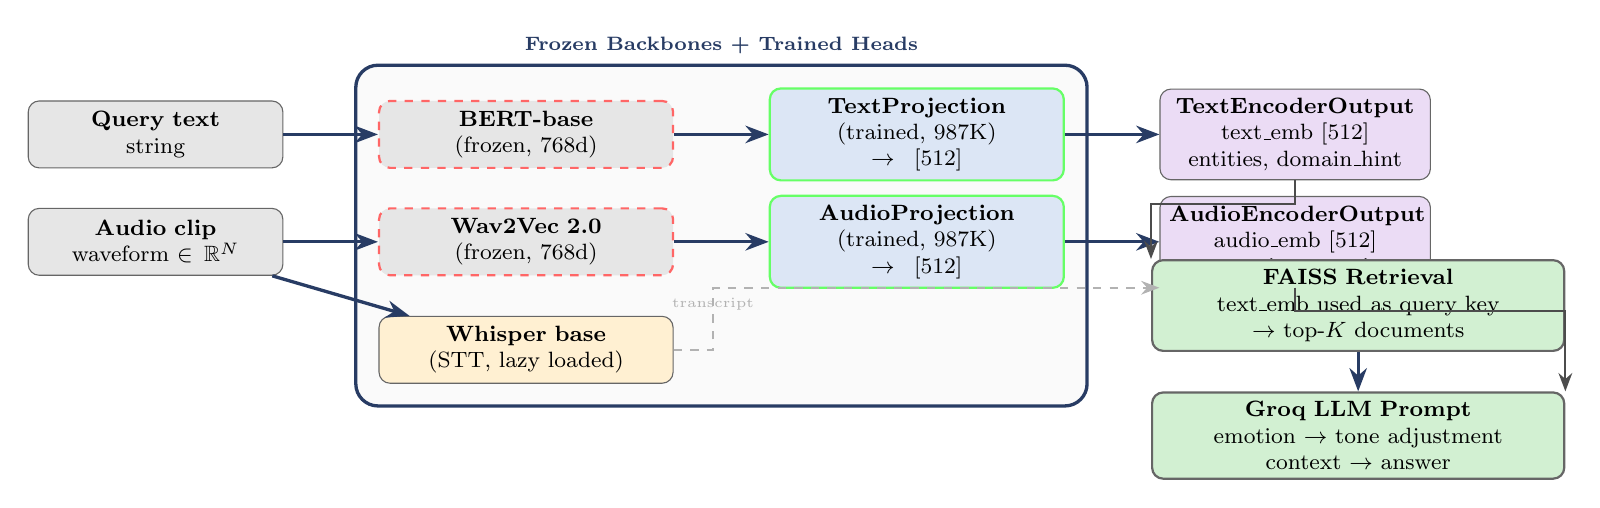
\begin{tikzpicture}[node distance=0.7cm and 1.2cm]

  \node[graynode,text width=3cm] (qt) {\textbf{Query text}\\string};
  \node[graynode,text width=3cm, below=0.5cm of qt] (qa)
      {\textbf{Audio clip}\\waveform $\in \mathbb{R}^N$};

  \node[frozennode,text width=3.5cm, right=1.2cm of qt] (bert)
      {\textbf{BERT-base}\\(frozen, 768d)};
  \node[frozennode,text width=3.5cm, right=1.2cm of qa] (wav)
      {\textbf{Wav2Vec 2.0}\\(frozen, 768d)};
  \node[whisnode,text width=3.5cm, below=0.5cm of wav] (whisper)
      {\textbf{Whisper base}\\(STT, lazy loaded)};

  \node[trainnode,text width=3.5cm, right=1.2cm of bert] (tproj)
      {\textbf{TextProjection}\\(trained, 987K)\\$\to [512]$};
  \node[trainnode,text width=3.5cm, right=1.2cm of wav] (aproj)
      {\textbf{AudioProjection}\\(trained, 987K)\\$\to [512]$};

  \node[outnode,text width=3.2cm, right=1.2cm of tproj] (te)
      {\textbf{TextEncoderOutput}\\text\_emb $[512]$\\entities, domain\_hint};
  \node[outnode,text width=3.2cm, right=1.2cm of aproj] (ae)
      {\textbf{AudioEncoderOutput}\\audio\_emb $[512]$\\transcript, emotion};

  \node[greennode,text width=5cm, below=1.0cm of te, xshift=0.8cm] (faiss)
      {\textbf{FAISS Retrieval}\\text\_emb used as query key\\$\to$ top-$K$ documents};
  \node[greennode,text width=5cm, below=0.5cm of faiss] (llm)
      {\textbf{Groq LLM Prompt}\\emotion $\to$ tone adjustment\\context $\to$ answer};

  \draw[thkarr] (qt) -- (bert);
  \draw[thkarr] (qa) -- (wav);
  \draw[thkarr] (qa) -- (whisper);
  \draw[thkarr] (bert) -- (tproj);
  \draw[thkarr] (wav) -- (aproj);
  \draw[thkarr] (tproj) -- (te);
  \draw[thkarr] (aproj) -- (ae);
  \draw[arr] (te.south) -- ++(0,-0.3) -| (faiss.north west);
  \draw[arr] (ae.south) -- ++(0,-0.3) -| (llm.north east);
  \draw[thkarr] (faiss) -- (llm);
  \draw[dasharr] (whisper.east) -- ++(0.5,0) |- (ae.south west)
      node[midway,below,font=\tiny]{transcript};

  \begin{pgfonlayer}{background}
    \node[basebox,fill=cGray!20,draw=cDark,very thick,rounded corners=8pt,
          fit=(bert)(wav)(whisper)(tproj)(aproj),inner sep=8pt,
          label={[font=\scriptsize\bfseries,text=cDark]above:Frozen Backbones + Trained Heads}] {};
  \end{pgfonlayer}

\end{tikzpicture}
\caption{Full module-level data flow of \texttt{encoders.py}.
Dashed borders = frozen; solid green borders = trained projection heads.}
\label{fig:module_flow}
\end{figure}

\subsection{Imports}

\begin{lstlisting}[caption={Module-level imports}]
import os
from abc import ABC, abstractmethod
from dataclasses import dataclass
from typing import Optional

import torch
import torch.nn as nn
import torch.nn.functional as F
\end{lstlisting}

\begin{remark}[Plain-language]
Think of each encoder as a language translator.
Raw text, audio waveforms, and video frames each ``speak a different language.''
The projection heads are learned dictionaries that convert each language into the
\emph{same universal language} — a 512-number vector — so the system can
compare them directly with dot products.
The imports bring in the tools: PyTorch for neural network layers (\texttt{nn}),
maths operations (\texttt{F}), and abstract class machinery (\texttt{ABC}).
\end{remark}

% ══════════════════════════════════════════════════
\section{Section 1: \texttt{TextProjection} — BERT $\to$ 512-d Shared Space}
% ══════════════════════════════════════════════════

\subsection{Code}

\begin{lstlisting}[caption={\texttt{TextProjection} class}]
class TextProjection(nn.Module):
    """
    BERT 768d -> proj -> 512d shared space.
    Checkpoint keys: proj.0.weight, proj.2.weight, proj.3.weight, norm.weight
    """
    def __init__(self, bert_dim: int = 768, embed_dim: int = 512):
        super().__init__()
        self.proj = nn.Sequential(
            nn.Linear(bert_dim, bert_dim),   # proj.0
            nn.GELU(),                        # proj.1
            nn.LayerNorm(bert_dim),           # proj.2
            nn.Linear(bert_dim, embed_dim),   # proj.3
        )
        self.norm = nn.LayerNorm(embed_dim)

    def forward(self, x: torch.Tensor) -> torch.Tensor:
        return F.normalize(self.norm(self.proj(x)), p=2, dim=1)
\end{lstlisting}

\subsection{Mathematical Definition}

Let $\mathbf{h} \in \mathbb{R}^{768}$ be the mean-pooled BERT hidden state.
The projection applies a two-layer MLP with normalisation:

\[
  \mathbf{z}_1 = W_1\,\mathbf{h} + \mathbf{b}_1,
  \quad W_1 \in \mathbb{R}^{768 \times 768}
\]
\[
  \mathbf{z}_2 = \text{GELU}(\mathbf{z}_1)
\]
\[
  \mathbf{z}_3 = \text{LayerNorm}_{768}(\mathbf{z}_2)
\]
\[
  \mathbf{z}_4 = W_2\,\mathbf{z}_3 + \mathbf{b}_2,
  \quad W_2 \in \mathbb{R}^{512 \times 768}
\]
\[
  \mathbf{z}_5 = \text{LayerNorm}_{512}(\mathbf{z}_4)
\]
\[
  \boxed{
    \mathbf{e}_{\text{text}} = \frac{\mathbf{z}_5}{\|\mathbf{z}_5\|_2}
    \in \mathbb{S}^{511}
  }
\]

\subsection{Component Definitions}

\begin{definition}[GELU Activation]
\[
  \text{GELU}(x) = x \cdot \Phi(x) \approx x \cdot \sigma(1.702\,x)
\]
where $\Phi$ is the standard normal CDF.
GELU is smoother than ReLU (no hard zero for negative inputs), which helps
gradient flow through the first linear layer.
\end{definition}

\begin{definition}[Layer Normalisation]
For $\mathbf{v} \in \mathbb{R}^d$:
\[
  \text{LayerNorm}(\mathbf{v})
  = \boldsymbol{\gamma} \odot
    \frac{\mathbf{v} - \mu}{\sqrt{\sigma^2 + \varepsilon}}
    + \boldsymbol{\beta}
\]
where $\mu = \frac{1}{d}\sum_i v_i$,
$\sigma^2 = \frac{1}{d}\sum_i (v_i - \mu)^2$,
$\varepsilon = 10^{-5}$, and $\boldsymbol{\gamma}, \boldsymbol{\beta}$ are
learned per-element scale and shift parameters.
LayerNorm stabilises training by normalising the distribution of
activations within each sample before the next linear layer.
\end{definition}

\subsection{Architecture Diagram}

\begin{figure}[H]
\centering
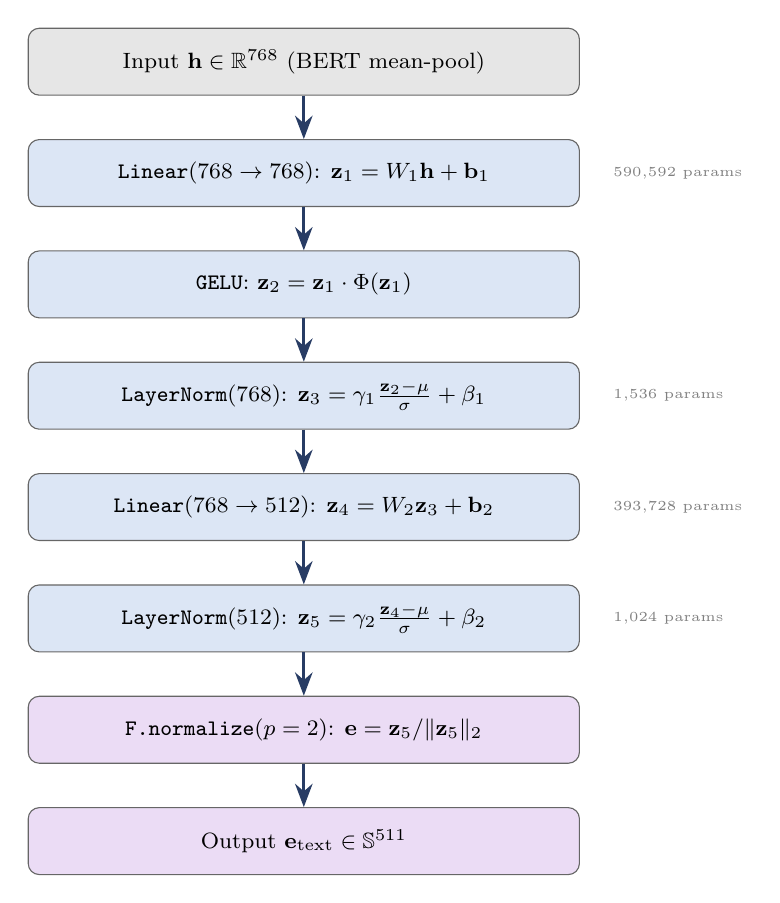
\begin{tikzpicture}[node distance=0.55cm]
  \node[graynode,minimum width=7cm] (inp)
      {Input $\mathbf{h} \in \mathbb{R}^{768}$ (BERT mean-pool)};
  \node[bluenode,minimum width=7cm,below=of inp] (l1)
      {\texttt{Linear}$(768 \to 768)$: $\mathbf{z}_1 = W_1\mathbf{h} + \mathbf{b}_1$};
  \node[bluenode,minimum width=7cm,below=of l1] (gelu)
      {\texttt{GELU}: $\mathbf{z}_2 = \mathbf{z}_1 \cdot \Phi(\mathbf{z}_1)$};
  \node[bluenode,minimum width=7cm,below=of gelu] (ln1)
      {\texttt{LayerNorm}$(768)$: $\mathbf{z}_3 = \gamma_1 \frac{\mathbf{z}_2-\mu}{\sigma} + \beta_1$};
  \node[bluenode,minimum width=7cm,below=of ln1] (l2)
      {\texttt{Linear}$(768 \to 512)$: $\mathbf{z}_4 = W_2\mathbf{z}_3 + \mathbf{b}_2$};
  \node[bluenode,minimum width=7cm,below=of l2] (ln2)
      {\texttt{LayerNorm}$(512)$: $\mathbf{z}_5 = \gamma_2 \frac{\mathbf{z}_4-\mu}{\sigma} + \beta_2$};
  \node[outnode,minimum width=7cm,below=of ln2] (l2n)
      {\texttt{F.normalize}$(p=2)$: $\mathbf{e} = \mathbf{z}_5 / \|\mathbf{z}_5\|_2$};
  \node[outnode,minimum width=7cm,below=of l2n] (out)
      {Output $\mathbf{e}_{\text{text}} \in \mathbb{S}^{511}$};

  \foreach \from/\to in {inp/l1,l1/gelu,gelu/ln1,ln1/l2,l2/ln2,ln2/l2n,l2n/out}
    \draw[thkarr] (\from) -- (\to);

  \node[font=\tiny,gray,right=0.3cm of l1]  {$590{,}592$ params};
  \node[font=\tiny,gray,right=0.3cm of ln1] {$1{,}536$ params};
  \node[font=\tiny,gray,right=0.3cm of l2]  {$393{,}728$ params};
  \node[font=\tiny,gray,right=0.3cm of ln2] {$1{,}024$ params};
\end{tikzpicture}
\caption{\texttt{TextProjection} layer-by-layer architecture with parameter counts.}
\label{fig:textproj}
\end{figure}

\subsection{Algorithm}

\begin{algorithm}[H]
\caption{\texttt{TextProjection.forward}($\mathbf{h}$)}
\label{alg:textproj}
\begin{algorithmic}[1]
\Require $\mathbf{h} \in \mathbb{R}^{B \times 768}$ (batch of BERT mean-pool vectors)
\Ensure $\mathbf{e} \in \mathbb{R}^{B \times 512}$ (unit-norm embeddings on $\mathbb{S}^{511}$)
\State $\mathbf{z}_1 \gets \text{Linear}_{768 \to 768}(\mathbf{h})$
       \Comment{Same-dim expansion}
\State $\mathbf{z}_2 \gets \text{GELU}(\mathbf{z}_1)$
       \Comment{Smooth non-linear activation}
\State $\mathbf{z}_3 \gets \text{LayerNorm}_{768}(\mathbf{z}_2)$
       \Comment{Stabilise scale}
\State $\mathbf{z}_4 \gets \text{Linear}_{768 \to 512}(\mathbf{z}_3)$
       \Comment{Project to shared dimension}
\State $\mathbf{z}_5 \gets \text{LayerNorm}_{512}(\mathbf{z}_4)$
       \Comment{Stabilise before normalisation}
\State $\mathbf{e} \gets \mathbf{z}_5 \;/\; \|\mathbf{z}_5\|_2$
       \Comment{L2-normalise $\to$ unit hypersphere}
\State \Return $\mathbf{e}$
\end{algorithmic}
\end{algorithm}

\subsection{Parameter Count}

\begin{table}[H]
\centering
\caption{\texttt{TextProjection} trainable parameters}
\begin{tabular}{lrc}
\toprule
Layer & Parameters & Formula \\
\midrule
\texttt{Linear}$(768 \to 768)$ & 590,592 & $768^2 + 768$ \\
\texttt{LayerNorm}$(768)$       & 1,536   & $2 \times 768$ \\
\texttt{Linear}$(768 \to 512)$ & 393,728 & $768 \times 512 + 512$ \\
\texttt{LayerNorm}$(512)$       & 1,024   & $2 \times 512$ \\
\midrule
\textbf{Total} & \textbf{$\approx$987K} & \\
\bottomrule
\end{tabular}
\end{table}

\begin{remark}[Plain-language]
Imagine BERT gives you a 768-word description of a sentence.
\texttt{TextProjection} is like a skilled editor who rewrites that description
into a concise 512-word summary, then rescales it so every summary has exactly
the same ``volume'' (unit norm).
Now two summaries can be compared just by checking how similar their words are
(dot product), and that similarity score is always between $-1$ and $+1$.
\end{remark}

% ══════════════════════════════════════════════════
\section{Section 2: \texttt{AudioProjection} — Wav2Vec 2.0 $\to$ 512-d}
% ══════════════════════════════════════════════════

\subsection{Code}

\begin{lstlisting}[caption={\texttt{AudioProjection} class}]
class AudioProjection(nn.Module):
    """
    Wav2Vec 768d -> proj -> 512d shared space.
    Pipeline C architecture: 768->512 (correct Wav2Vec 2.0 base output dim).
    """
    def __init__(self, wav2vec_dim: int = 768, embed_dim: int = 512):
        super().__init__()
        self.proj = nn.Sequential(
            nn.Linear(wav2vec_dim, wav2vec_dim),
            nn.GELU(),
            nn.LayerNorm(wav2vec_dim),
            nn.Linear(wav2vec_dim, embed_dim),
        )
        self.norm = nn.LayerNorm(embed_dim)

    def forward(self, x: torch.Tensor) -> torch.Tensor:
        return F.normalize(self.norm(self.proj(x)), p=2, dim=1)
\end{lstlisting}

\subsection{Mathematical Definition}

Let $\mathbf{a} \in \mathbb{R}^{768}$ be the mean-pooled Wav2Vec 2.0 hidden state.
The architecture is \emph{structurally identical} to \texttt{TextProjection}:

\[
  \mathbf{e}_{\text{audio}}
  = \text{L2Norm}\!\left(
    \text{LN}_{512}\!\left(W_2\,
    \text{LN}_{768}\!\left(\text{GELU}(W_1\mathbf{a})\right)\right)\right)
  \in \mathbb{S}^{511}
\]

\subsection{Why Mean-Pool Wav2Vec Frames?}

Wav2Vec 2.0 outputs a \emph{sequence} of frames $\{F_t\}_{t=1}^T$,
one frame per $\approx$20 ms window at 16 kHz:

\[
  \mathbf{a} = \frac{1}{T}\sum_{t=1}^{T} F_t \in \mathbb{R}^{768}
\]

\begin{lemma}[Mean-Pool as Fixed-Size Summary]
For a clip of duration $D$ seconds at $f_s = 16{,}000$ Hz,
$T \approx D \times f_s / 320 \approx 50D$ frames.
Mean-pooling compresses this variable-length sequence to a fixed 768-d vector
regardless of clip length, directly analogous to BERT's mean-pool over tokens.
The emotion information is a \emph{global} property of the utterance
(not localised to one frame), so averaging over time is an appropriate compression.
\end{lemma}

\begin{lemma}[Shared-Space Alignment]
Because both \texttt{TextProjection} and \texttt{AudioProjection}:
\begin{enumerate}
  \item project into the same 512-dimensional space, and
  \item L2-normalise their outputs to $\mathbb{S}^{511}$,
\end{enumerate}
the dot product
$\mathbf{e}_{\text{text}} \cdot \mathbf{e}_{\text{audio}} \in [-1, 1]$
is a valid cosine similarity score directly comparable without any further
scaling.
This is trained via contrastive losses (InfoNCE / SupCon) in Pipelines A--D.
\end{lemma}

\begin{remark}[Plain-language]
Imagine two people who grew up speaking different languages (text vs audio).
\texttt{TextProjection} and \texttt{AudioProjection} are two separate
language schools that both teach the same universal sign language.
After graduation, the two people can sign to each other directly —
their ``signs'' live in the same 512-sign dictionary.
\end{remark}

% ══════════════════════════════════════════════════
\section{Section 3: \texttt{\_load\_checkpoint} — Safe Checkpoint Loader}
% ══════════════════════════════════════════════════

\subsection{Code}

\begin{lstlisting}[caption={\texttt{\_load\_checkpoint} function}]
def _load_checkpoint(path: str, device: torch.device):
    """
    Load a checkpoint file and unwrap if needed.
    Returns: (state_dict, full_checkpoint_dict)
    """
    ckpt = torch.load(path, map_location=device, weights_only=False)
    if isinstance(ckpt, dict) and "model_state_dict" in ckpt:
        return ckpt["model_state_dict"], ckpt
    return ckpt, {}
\end{lstlisting}

\subsection{Problem Statement and Algorithm}

PyTorch checkpoints saved with \texttt{torch.save()} can take two forms:

\begin{table}[H]
\centering
\caption{Two PyTorch checkpoint formats}
\begin{tabularx}{\textwidth}{lXX}
\toprule
Format & Structure & Created by \\
\midrule
\textbf{Wrapped} & \texttt{\{'model\_state\_dict': OrderedDict, 'epoch': int, \ldots\}} & Training loop with metadata \\
\textbf{Raw}     & \texttt{OrderedDict} directly & \texttt{torch.save(model.state\_dict(), path)} \\
\bottomrule
\end{tabularx}
\end{table}

\begin{algorithm}[H]
\caption{\texttt{\_load\_checkpoint}(path, device)}
\label{alg:load_ckpt}
\begin{algorithmic}[1]
\Require \texttt{path}: filesystem path to \texttt{.pt}/\texttt{.pth} file;
         \texttt{device}: \texttt{torch.device}
\Ensure (\texttt{state\_dict}, \texttt{meta\_dict}) tuple
\State $\textit{ckpt} \gets \texttt{torch.load}(\textit{path},\;
       \text{map\_location}=\textit{device},\; \text{weights\_only}=\textsc{False})$
\If{$\textit{ckpt}$ is a \texttt{dict} \textbf{and}
    $\texttt{"model\_state\_dict"} \in \textit{ckpt}$}
  \State \Return $(\textit{ckpt}[\texttt{"model\_state\_dict"}],\; \textit{ckpt})$
         \Comment{Wrapped format: unwrap + keep metadata}
\Else
  \State \Return $(\textit{ckpt},\; \{\})$
         \Comment{Raw state dict: use as-is, empty meta}
\EndIf
\end{algorithmic}
\end{algorithm}

\subsection{Flowchart}

\begin{figure}[H]
\centering
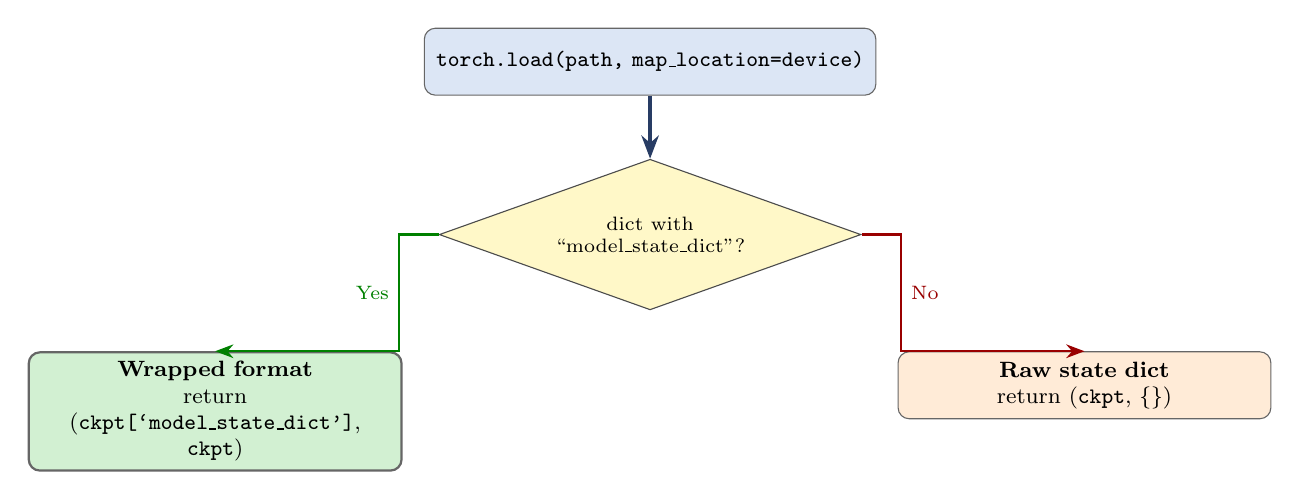
\begin{tikzpicture}[node distance=0.8cm]
  \node[bluenode,text width=5.5cm] (load)
      {\texttt{torch.load(path, map\_location=device)}};
  \node[decnode,text width=3.2cm, below=of load] (check)
      {dict with\\``model\_state\_dict''?};
  \node[greennode,text width=4.5cm, below left=1.0cm and 1.8cm of check] (wrap)
      {\textbf{Wrapped format}\\return (\texttt{ckpt[`model\_state\_dict']},\\
       \texttt{ckpt})};
  \node[orangenode,text width=4.5cm, below right=1.0cm and 1.8cm of check] (raw)
      {\textbf{Raw state dict}\\return (\texttt{ckpt}, \texttt{\{\}})};

  \draw[thkarr] (load) -- (check);
  \draw[grnarr] (check.west) -- ++(-0.5,0) |- (wrap.north)
      node[near start,left,font=\scriptsize]{Yes};
  \draw[redarr] (check.east) -- ++(0.5,0) |- (raw.north)
      node[near start,right,font=\scriptsize]{No};
\end{tikzpicture}
\caption{Control flow of \texttt{\_load\_checkpoint}: handles both
wrapped and raw checkpoint formats transparently.}
\label{fig:load_ckpt}
\end{figure}

\begin{proposition}[\texttt{map\_location} — Cross-Device Loading]
When loading a checkpoint saved on GPU onto a CPU machine (or vice versa):
\[
  \text{map\_location} = \textit{device}
  \implies \forall\, t \in \text{state\_dict}:\;
  t.\text{device} \leftarrow \textit{device}
\]
Without \texttt{map\_location}, PyTorch restores tensors to the
\emph{original} device (e.g., \texttt{cuda:0}), failing on CPU-only machines.
\end{proposition}

\begin{remark}[Plain-language: \texttt{weights\_only=False}]
PyTorch 2.6 defaults to \texttt{weights\_only=True}, which blocks arbitrary
Python objects inside \texttt{.pt} files.
Month 2 checkpoints were saved with older PyTorch and may contain non-tensor
objects (loss lists, epoch counters), so \texttt{weights\_only=False} is required.
Think of it like opening a zip file from a trusted colleague:
normally the OS asks ``are you sure?'' for unknown file types.
\texttt{weights\_only=False} says ``yes, I trust this file'' — safe here
because we generated these checkpoints ourselves.
\end{remark}

% ══════════════════════════════════════════════════
\section{Section 4: Data Contracts — \texttt{AudioEncoderOutput} \& \texttt{TextEncoderOutput}}
% ══════════════════════════════════════════════════

\subsection{Code}

\begin{lstlisting}[caption={Output dataclass contracts}]
@dataclass
class AudioEncoderOutput:
    transcript:   str
    emotion:      str
    emotion_conf: float
    audio_emb:    torch.Tensor
    raw_audio:    Optional[torch.Tensor] = None

@dataclass
class TextEncoderOutput:
    text:        str
    text_emb:    torch.Tensor
    entities:    list
    domain_hint: Optional[str] = None  # "medical" if >=2 hits
\end{lstlisting}

\subsection{Field Specifications}

\begin{table}[H]
\centering
\caption{\texttt{AudioEncoderOutput} fields}
\begin{tabularx}{\textwidth}{llXl}
\toprule
Field & Type & Description & Source \\
\midrule
\texttt{transcript}   & \texttt{str} & Whisper STT transcription & Whisper base \\
\texttt{emotion}      & \texttt{str} & One of 8 RAVDESS classes & Centroid-NN \\
\texttt{emotion\_conf}& \texttt{float} & Cosine sim to winning centroid $\in [-1,1]$ & Centroid-NN \\
\texttt{audio\_emb}   & \texttt{Tensor[512]} & L2-normalised projected embedding & AudioProjection \\
\texttt{raw\_audio}   & \texttt{Tensor?} & Original waveform (optional) & Input \\
\bottomrule
\end{tabularx}
\end{table}

\begin{table}[H]
\centering
\caption{\texttt{TextEncoderOutput} fields}
\begin{tabularx}{\textwidth}{llXl}
\toprule
Field & Type & Description & Source \\
\midrule
\texttt{text}        & \texttt{str} & Original query string & Input \\
\texttt{text\_emb}   & \texttt{Tensor[512]} & L2-normalised projected embedding & TextProjection \\
\texttt{entities}    & \texttt{list[str]} & spaCy NER + noun chunks & spaCy \\
\texttt{domain\_hint}& \texttt{str?} & \texttt{"medical"} if $\geq 2$ MEDICAL\_TERMS hit & Rule-based \\
\bottomrule
\end{tabularx}
\end{table}

\begin{theorem}[Dependency Inversion via Output Contracts]
By separating the output container from the encoder implementation,
any downstream module (FAISS retriever, KG re-ranker, LLM prompt builder, TTS)
can depend on \texttt{AudioEncoderOutput} or \texttt{TextEncoderOutput}
\emph{without} importing or knowing about Wav2Vec 2.0, Whisper,
\texttt{AudioProjection}, or \texttt{TextProjection}.
This is the \textbf{Dependency Inversion Principle}: high-level modules
depend on abstractions (data contracts), not concrete implementations.
\end{theorem}

\begin{remark}[Plain-language]
Think of the output dataclasses as standardised forms with labelled boxes.
Every encoder fills out the same form, so the rest of the system always
knows exactly where to find the transcript, the emotion, and the embedding —
no guessing about dictionary keys.
Just as a doctor's report always has the same sections regardless of which
doctor wrote it, these dataclasses ensure consistent structure.
\end{remark}

% ══════════════════════════════════════════════════
\section{Section 5: Abstract Base Classes — \texttt{BaseAudioEncoder} \& \texttt{BaseTextEncoder}}
% ══════════════════════════════════════════════════

\subsection{Code}

\begin{lstlisting}[caption={Abstract Base Classes}]
class BaseAudioEncoder(ABC):
    @abstractmethod
    def encode(self, audio: torch.Tensor,
               sample_rate: int = 16000) -> AudioEncoderOutput: pass
    @abstractmethod
    def load_weights(self, weights_path: str,
                     centroids_path: str = None) -> None: pass

class BaseTextEncoder(ABC):
    @abstractmethod
    def encode(self, text: str) -> TextEncoderOutput: pass
    @abstractmethod
    def load_weights(self, weights_path: str) -> None: pass
\end{lstlisting}

\subsection{ABC Hierarchy Diagram}

\begin{figure}[H]
\centering
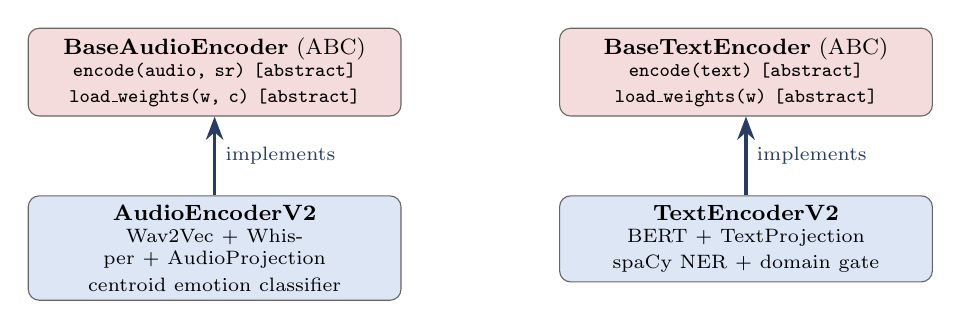
\begin{tikzpicture}[node distance=0.9cm and 1.5cm]

  \node[warnnode,text width=4.5cm] (bae)
      {\textbf{BaseAudioEncoder} (ABC)\\
       \scriptsize \texttt{encode(audio, sr) [abstract]}\\
       \texttt{load\_weights(w, c) [abstract]}};

  \node[warnnode,text width=4.5cm, right=2.0cm of bae] (bte)
      {\textbf{BaseTextEncoder} (ABC)\\
       \scriptsize \texttt{encode(text) [abstract]}\\
       \texttt{load\_weights(w) [abstract]}};

  \node[bluenode,text width=4.5cm, below=1.0cm of bae] (aev2)
      {\textbf{AudioEncoderV2}\\
       \scriptsize Wav2Vec + Whisper + AudioProjection\\
       centroid emotion classifier};

  \node[bluenode,text width=4.5cm, below=1.0cm of bte] (tev2)
      {\textbf{TextEncoderV2}\\
       \scriptsize BERT + TextProjection\\
       spaCy NER + domain gate};

  \draw[thkarr] (aev2.north) -- (bae.south)
      node[midway,right,font=\scriptsize]{implements};
  \draw[thkarr] (tev2.north) -- (bte.south)
      node[midway,right,font=\scriptsize]{implements};

\end{tikzpicture}
\caption{ABC hierarchy. Python raises \texttt{TypeError} at instantiation
if any \texttt{@abstractmethod} is not implemented.}
\label{fig:abc}
\end{figure}

\begin{theorem}[Liskov Substitution Principle]
For any module $M$ that accepts a \texttt{BaseTextEncoder} instance $e$,
replacing $e$ with any concrete subclass $e'$ (e.g., \texttt{TextEncoderV2},
a future \texttt{TextEncoderV3} using a different backbone) must not break
$M$'s behaviour, provided $e'$ honours the method signatures and output types.
This means future encoder upgrades are \textbf{drop-in replacements} without
modifying any downstream code.
\end{theorem}

\begin{remark}[Plain-language]
An ABC is a job description.
The description says: ``this role must be able to: (1) encode inputs,
(2) load weights.'' It does \emph{not} say \emph{how} to do those things —
that is left to the person (concrete class) who fills the role.
Python runtime acts as HR: it will refuse to instantiate anyone
(\texttt{TypeError}) who cannot do both tasks.
\end{remark}

% ══════════════════════════════════════════════════
\section{Section 6: \texttt{TextEncoderV2} — Full Text Encoding Pipeline}
% ══════════════════════════════════════════════════

\subsection{Code}

\begin{lstlisting}[caption={\texttt{TextEncoderV2} class}]
class TextEncoderV2(BaseTextEncoder):
    MEDICAL_TERMS = {
        "pneumonia", "effusion", "atelectasis", "cardiomegaly",
        "consolidation", "opacity", "bilateral", "pleural", "nodule",
        "mass", "fracture", "edema", "pneumothorax", "fibrosis",
        "emphysema", "radiology", "chest", "xray", "x-ray", "ct scan",
        "mri", "ultrasound", "lesion", "tumor", "malignant", "benign",
        "biopsy", "diagnosis", "clinical", "patient", "scan",   # 31 terms
    }

    def encode(self, text: str) -> TextEncoderOutput:
        inputs = self.tokenizer(text, return_tensors="pt", padding=True,
                                truncation=True, max_length=128).to(self.device)
        bert_emb = self.bert(**inputs).last_hidden_state.mean(dim=1)
        text_emb = self.projection(bert_emb).squeeze(0).cpu()
        doc = self.nlp(text)
        entities = list(set(
            [chunk.text.lower() for chunk in doc.noun_chunks] +
            [ent.text.lower() for ent in doc.ents]
        ))
        lower = text.lower()
        medical_hits = sum(1 for t in self.MEDICAL_TERMS if t in lower)
        domain_hint = "medical" if medical_hits >= 2 else None
        return TextEncoderOutput(text=text, text_emb=text_emb,
                                 entities=entities, domain_hint=domain_hint)
\end{lstlisting}

\subsection{Full Mathematical Pipeline}

Given input string $s$:

\textbf{Step 1 — Tokenisation:}
\[
  (x_{\text{ids}}, x_{\text{mask}}) = \text{BertTokenizer}(s,\; \text{max\_len}=128)
\]

\textbf{Step 2 — BERT Encoding (frozen):}
\[
  H = \text{BERT}_{\theta^*}(x_{\text{ids}}, x_{\text{mask}})
  \in \mathbb{R}^{L \times 768}
\]
where $L \leq 128$ is the token count and $\theta^*$ denotes frozen parameters.

\textbf{Step 3 — Mean Pooling:}
\[
  \mathbf{h} = \frac{1}{L}\sum_{\ell=1}^{L} H_\ell \in \mathbb{R}^{768}
\]

\textbf{Step 4 — Projection:}
\[
  \mathbf{e}_{\text{text}} = \text{TextProjection}(\mathbf{h}) \in \mathbb{S}^{511}
\]

\textbf{Step 5 — NER \& Domain Detection:}
\[
  \mathcal{E} = \text{spaCy\_NER}(s) \cup \text{NounChunks}(s)
\]
\[
  \text{domain\_hint} = \begin{cases}
    \texttt{"medical"} & \text{if } \displaystyle\sum_{t \in \mathcal{T}_{\text{med}}}
                         \mathbf{1}[t \subseteq s_{\text{lower}}] \geq 2 \\
    \texttt{None}      & \text{otherwise}
  \end{cases}
\]
where $\mathcal{T}_{\text{med}}$ is the 31-term \texttt{MEDICAL\_TERMS} set.

\subsection{Medical Domain Gate}

The domain gate is a \textbf{bag-of-words classifier} — the simplest possible:

\begin{definition}[Bag-of-Words Domain Classifier]
\[
  \hat{y} = \begin{cases}
    1 & \displaystyle\sum_{t \in \mathcal{T}} \mathbf{1}[t \subseteq s] \geq \tau \\
    0 & \text{otherwise}
  \end{cases}
\]
with threshold $\tau = 2$.
\end{definition}

\begin{proposition}[Threshold $\tau = 2$ Prevents False Positives]
A single medical word can appear innocuously
(e.g., ``my chest hurts'' $\to$ 1 hit $\to$ no trigger).
Two or more medical terms
(e.g., ``chest X-ray shows opacity'' $\to$ 3 hits $\to$ medical domain)
provide stronger evidence of a clinical query,
reducing false domain-switch events that would inappropriately apply the
stricter medical confidence threshold.
\end{proposition}

\subsection{TextEncoderV2 Full Pipeline Flowchart}

\begin{figure}[H]
\centering
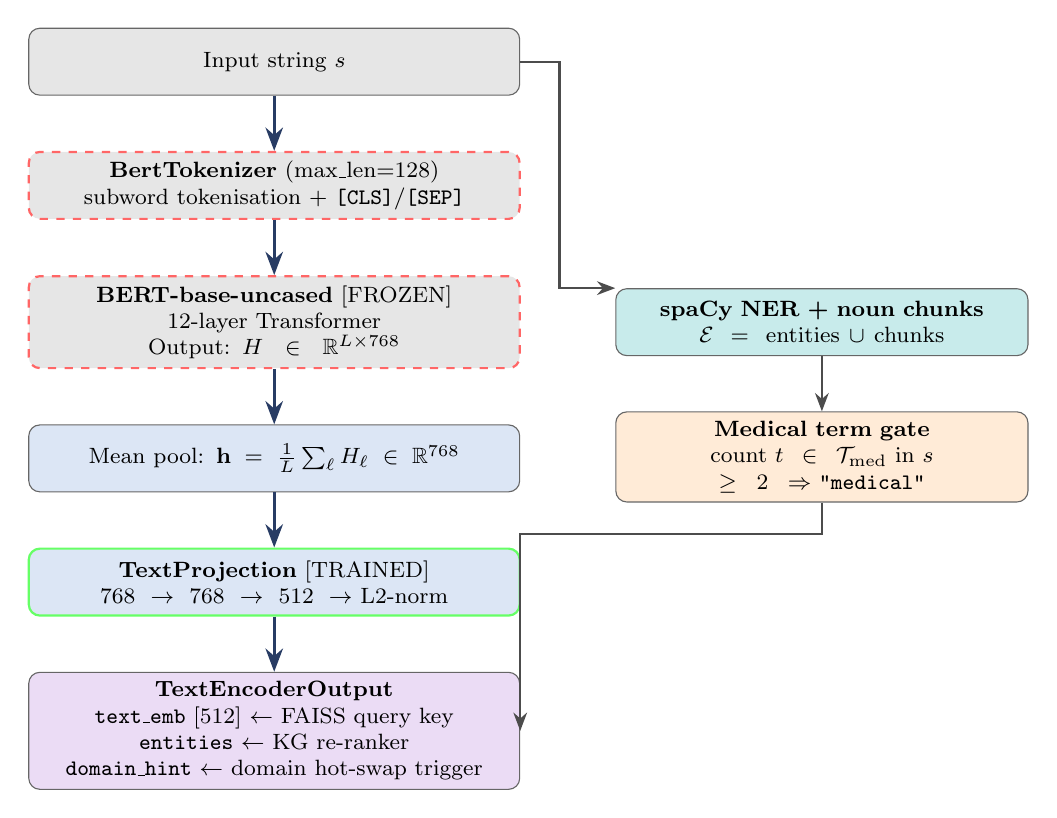
\begin{tikzpicture}[node distance=0.7cm]

  \node[graynode,text width=6cm] (inp) {Input string $s$};

  \node[frozennode,text width=6cm, below=of inp] (tok)
      {\textbf{BertTokenizer} (max\_len=128)\\subword tokenisation + \texttt{[CLS]}/\texttt{[SEP]}};

  \node[frozennode,text width=6cm, below=of tok] (bert)
      {\textbf{BERT-base-uncased} [FROZEN]\\12-layer Transformer\\Output: $H \in \mathbb{R}^{L \times 768}$};

  \node[bluenode,text width=6cm, below=of bert] (mp)
      {Mean pool: $\mathbf{h} = \frac{1}{L}\sum_\ell H_\ell \in \mathbb{R}^{768}$};

  \node[trainnode,text width=6cm, below=of mp] (tproj)
      {\textbf{TextProjection} [TRAINED]\\$768 \to 768 \to 512 \to$ L2-norm};

  % Fork: NER branch alongside projection
  \node[tealnode,text width=5cm, right=1.2cm of bert] (ner)
      {\textbf{spaCy NER + noun chunks}\\$\mathcal{E} = \text{entities} \cup \text{chunks}$};
  \node[orangenode,text width=5cm, below=0.7cm of ner] (gate)
      {\textbf{Medical term gate}\\count $t \in \mathcal{T}_{\text{med}}$ in $s$\\
       $\geq 2 \Rightarrow$ \texttt{"medical"}};

  \node[outnode,text width=6cm, below=of tproj] (out)
      {\textbf{TextEncoderOutput}\\
       \texttt{text\_emb $[512]$} $\leftarrow$ FAISS query key\\
       \texttt{entities} $\leftarrow$ KG re-ranker\\
       \texttt{domain\_hint} $\leftarrow$ domain hot-swap trigger};

  \draw[thkarr] (inp) -- (tok);
  \draw[thkarr] (tok) -- (bert);
  \draw[thkarr] (bert) -- (mp);
  \draw[thkarr] (mp) -- (tproj);
  \draw[thkarr] (tproj) -- (out);
  \draw[arr] (inp.east) -- ++(0.5,0) |- (ner.north west);
  \draw[arr] (ner) -- (gate);
  \draw[arr] (gate.south) -- ++(0,-0.4) -| (out.east);

\end{tikzpicture}
\caption{\texttt{TextEncoderV2.encode()} full pipeline. The text string is
simultaneously encoded through BERT (left branch) and analysed by spaCy NER
(right branch). Both outputs are packed into \texttt{TextEncoderOutput}.}
\label{fig:textencv2}
\end{figure}

\subsection{Algorithms}

\begin{algorithm}[H]
\caption{\texttt{TextEncoderV2.encode}(text)}
\label{alg:textencode}
\begin{algorithmic}[1]
\Require \texttt{text}: raw query string
\Ensure \texttt{TextEncoderOutput}
\State $\textit{tokens} \gets \text{BertTokenizer}(\textit{text},
       \text{max\_len}=128, \text{truncate}=\text{True}).\textsc{to}(\textit{device})$
\State $H \gets \text{BERT}(\textit{tokens}).\texttt{last\_hidden\_state}$
       \Comment{$[1, L, 768]$}
\State $\mathbf{h} \gets H.\text{mean}(\text{dim}=1)$
       \Comment{$[1, 768]$}
\State $\mathbf{e} \gets \text{TextProjection}(\mathbf{h}).\text{squeeze}(0).\text{cpu}()$
       \Comment{$[512]$}
\State $\textit{doc} \gets \text{spaCy}(\textit{text})$
\State $\mathcal{E} \gets \{\textit{chunk.text.lower()} \mid \textit{chunk} \in \textit{doc.noun\_chunks}\}
       \cup \{\textit{ent.text.lower()} \mid \textit{ent} \in \textit{doc.ents}\}$
\State $n_{\text{hits}} \gets |\{t \in \mathcal{T}_{\text{med}} \mid t \subseteq \textit{text.lower()}\}|$
\State $\textit{hint} \gets \texttt{"medical"}$ if $n_{\text{hits}} \geq 2$ else \texttt{None}
\State \Return $\texttt{TextEncoderOutput}(\textit{text},\, \mathbf{e},\, \mathcal{E},\, \textit{hint})$
\end{algorithmic}
\end{algorithm}

\begin{algorithm}[H]
\caption{\texttt{TextEncoderV2.load\_weights}(weights\_path)}
\label{alg:textload}
\begin{algorithmic}[1]
\Require \texttt{weights\_path}: path to TextProjection checkpoint
\State $\textit{tokenizer} \gets \texttt{AutoTokenizer}(\texttt{"bert-base-uncased"})$
\State $\textit{bert} \gets \texttt{AutoModel}(\texttt{"bert-base-uncased"})$
\ForEach{$p \in \textit{bert}.\text{parameters}()$}
  \State $p.\text{requires\_grad} \gets \textsc{False}$
         \Comment{Freeze all BERT parameters}
\EndFor
\State $\textit{bert}.\text{eval}().\textsc{to}(\textit{device})$
\State $(\textit{state}, \textit{meta}) \gets \textsc{\_load\_checkpoint}(\textit{weights\_path}, \textit{device})$
\State $\textit{projection} \gets \text{TextProjection}().\textsc{to}(\textit{device})$
\State $\textit{projection}.\text{load\_state\_dict}(\textit{state})$
\State $\textit{projection}.\text{eval}()$
\State \textbf{try:} $\textit{nlp} \gets \text{spacy.load}(\textit{ner\_model\_name})$
\State \textbf{except OSError:} $\textit{nlp} \gets \text{spacy.load}(\texttt{"en\_core\_web\_sm"})$
       \Comment{Graceful NER fallback}
\end{algorithmic}
\end{algorithm}

\begin{proposition}[\texttt{@torch.no\_grad()} Memory Saving]
During inference, gradient computation is unnecessary.
\texttt{@torch.no\_grad()} disables the autograd tape, saving:
\[
  \Delta M \approx \sum_{\text{layer}} \|\text{activations}_{\text{layer}}\|
  \times 4\;\text{bytes}
\]
This approximately halves memory usage for large batches because no
intermediate activation tensors need to be retained for backpropagation.
\end{proposition}

\begin{remark}[Plain-language: full text pipeline]
\begin{enumerate}
  \item \textbf{Tokeniser}: cuts the sentence into subword pieces
    (``playing'' $\to$ ``play'' + ``\#\#ing'') and adds BERT bookends
    \texttt{[CLS]} and \texttt{[SEP]}.
  \item \textbf{BERT (frozen)}: reads all tokens at once using self-attention
    — each word ``looks at'' every other word. We freeze it: it is treated
    like a pre-built dictionary we are not allowed to edit.
  \item \textbf{Mean pool}: average all token vectors into one 768-number summary.
  \item \textbf{TextProjection}: squeeze the 768-number summary into 512 numbers
    and make its total length exactly 1 (unit-normalise).
  \item \textbf{NER}: spaCy spots named entities (``chest X-ray'' $\to$ entity).
  \item \textbf{Domain gate}: count medical buzzwords — if $\geq 2$ appear,
    flag as ``medical'' to hot-swap the retrieval backend.
\end{enumerate}
\end{remark}

% ══════════════════════════════════════════════════
\section{Section 7: \texttt{AudioEncoderV2} — Full Audio Encoding Pipeline}
% ══════════════════════════════════════════════════

\subsection{Code}

\begin{lstlisting}[caption={\texttt{AudioEncoderV2} class (condensed)}]
class AudioEncoderV2(BaseAudioEncoder):
    EMOTIONS = ["angry","calm","disgust","fearful",
                "happy","neutral","sad","surprised"]

    @torch.no_grad()
    def encode(self, audio, sample_rate=16000) -> AudioEncoderOutput:
        transcript = self.transcribe(audio, sample_rate)
        inputs = self.wav2vec_processor(audio.cpu().numpy(),
                     sampling_rate=16000, return_tensors="pt").to(self.device)
        wav2vec_out = self.wav2vec(**inputs).last_hidden_state.mean(dim=1)
        audio_emb = self.projection(wav2vec_out).squeeze(0).cpu()
        emotion, emotion_conf = "neutral", 0.0
        if self.emotion_centroids is not None:
            sims = F.cosine_similarity(
                audio_emb.unsqueeze(0), self.emotion_centroids.cpu(), dim=1)
            best_idx = sims.argmax().item()
            emotion = self.EMOTIONS[best_idx]
            emotion_conf = sims[best_idx].item()
        return AudioEncoderOutput(transcript, emotion, emotion_conf, audio_emb, audio)
\end{lstlisting}

\subsection{Full Mathematical Pipeline}

Given raw waveform $\mathbf{w} \in \mathbb{R}^N$ at 16 kHz:

\textbf{Step 1 — STT (Whisper):}
\[
  \text{transcript} = \text{Whisper}_{\text{base}}(\mathbf{w}) \in \Sigma^*
\]

\textbf{Step 2 — Wav2Vec Feature Extraction (frozen):}
\[
  F = \text{Wav2Vec2}_{\phi^*}(\mathbf{w}) \in \mathbb{R}^{T \times 768}
\]
where $T \approx N / 320$ (one frame per 20 ms at 16 kHz).

\textbf{Step 3 — Mean Pooling:}
\[
  \mathbf{a} = \frac{1}{T}\sum_{t=1}^{T} F_t \in \mathbb{R}^{768}
\]

\textbf{Step 4 — Audio Projection:}
\[
  \mathbf{e}_{\text{audio}} = \text{AudioProjection}(\mathbf{a}) \in \mathbb{S}^{511}
\]

\textbf{Step 5 — Emotion Classification via Centroid Matching:}

Let $C \in \mathbb{R}^{8 \times 512}$ be the pre-computed RAVDESS centroid matrix.
\[
  \hat{k} = \arg\max_{k \in \{0,\ldots,7\}}
  \cos(\mathbf{e}_{\text{audio}},\, C_k)
  = \arg\max_{k}\; \mathbf{e}_{\text{audio}} \cdot C_k
\]
\[
  \text{emotion} = \texttt{EMOTIONS}[\hat{k}], \qquad
  \text{conf} = \mathbf{e}_{\text{audio}} \cdot C_{\hat{k}}
\]

\subsection{Emotion Classes and Centroid Matrix}

\[
  \texttt{EMOTIONS} =
  [\text{angry}, \text{calm}, \text{disgust}, \text{fearful},
   \text{happy}, \text{neutral}, \text{sad}, \text{surprised}]
\]
\[
  C = \begin{bmatrix}
    \mathbf{c}_{\text{angry}} \\
    \mathbf{c}_{\text{calm}} \\
    \vdots \\
    \mathbf{c}_{\text{surprised}}
  \end{bmatrix} \in \mathbb{R}^{8 \times 512}
\]

Each centroid $\mathbf{c}_k$ was computed offline by
\texttt{build\_emotion\_centroids} (Section~8) and loaded once at startup.

\subsection{Lazy Whisper Loading}

\begin{definition}[Lazy Initialisation]
A resource is not created until first needed.
Formally, let $\mathcal{W} = \bot$ at startup.
On first call to \texttt{\_load\_whisper()}, $\mathcal{W} \leftarrow \text{Whisper.load}(\cdot)$.
Subsequent calls skip loading because $\mathcal{W} \neq \bot$.
\[
  \texttt{\_load\_whisper}() =
  \begin{cases}
    \text{Whisper.load}(\texttt{"base"}) \to \mathcal{W}
    & \text{if } \mathcal{W} = \bot \\
    \text{no-op} & \text{if } \mathcal{W} \neq \bot
  \end{cases}
\]
\end{definition}

\begin{proposition}[Lazy Loading Saves $\approx$1 GB VRAM]
Whisper base requires $\approx$1 GB VRAM.
Text-only queries (no audio) never trigger \texttt{\_load\_whisper()},
so Whisper is never loaded for those queries.
For a system that handles mixed text/audio queries, this saves
$\approx$1 GB VRAM in text-only sessions.
\end{proposition}

\subsection{Sample Rate Resampling}

If the input sample rate $r \neq 16000$ Hz:
\[
  \mathbf{w}_{16k} =
  \text{librosa.resample}(\mathbf{w},\; r_{\text{orig}} \to 16000)
\]

\begin{axiom}[16 kHz Requirement]
Both Whisper and Wav2Vec 2.0 were pre-trained at exactly 16 kHz.
Feeding audio at a different sample rate would compress or stretch phonemes,
degrading both transcription accuracy and audio embedding quality.
All audio inputs \emph{must} be resampled to 16 kHz before processing.
\end{axiom}

\subsection{AudioEncoderV2 Full Pipeline Flowchart}

\begin{figure}[H]
\centering
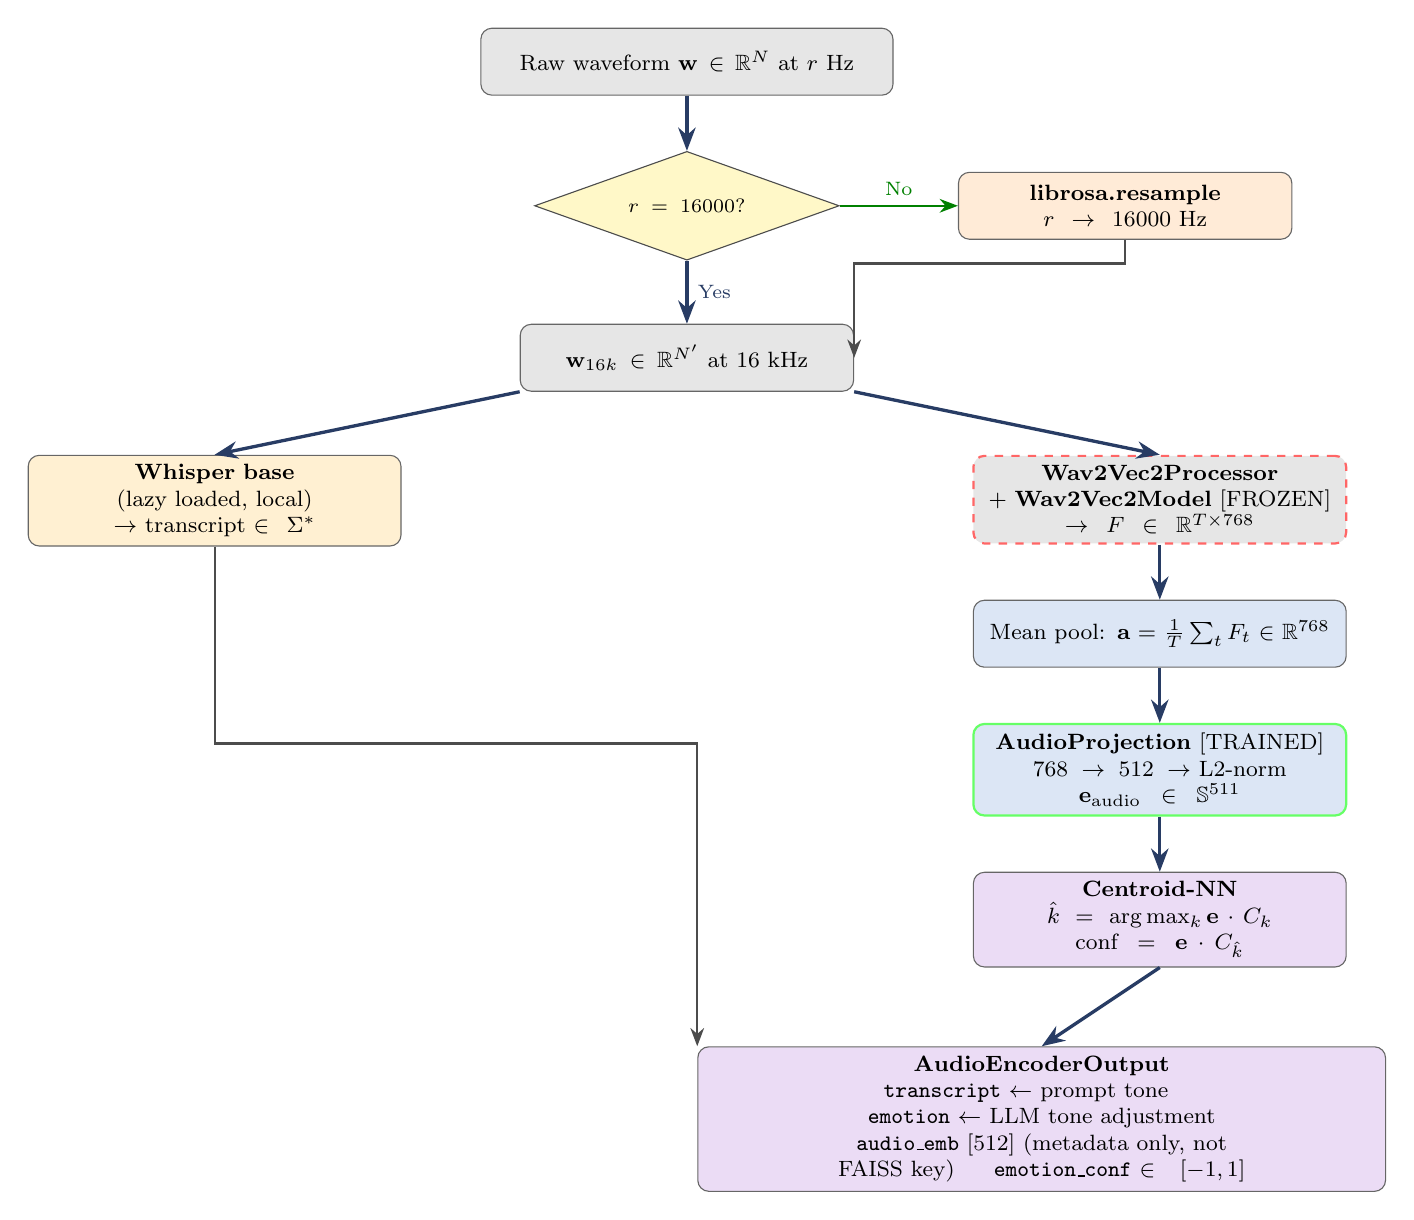
\begin{tikzpicture}[node distance=0.7cm and 1.0cm]

  \node[graynode,text width=5cm] (inp)
      {Raw waveform $\mathbf{w} \in \mathbb{R}^N$ at $r$ Hz};

  % Resample decision
  \node[decnode, text width=2.5cm, below=of inp] (sr_dec)
      {$r = 16000$?};
  \node[orangenode,text width=4cm, right=1.5cm of sr_dec] (resamp)
      {\textbf{librosa.resample}\\$r \to 16000$ Hz};
  \node[graynode,text width=4cm, below=0.8cm of sr_dec] (w16)
      {$\mathbf{w}_{16k} \in \mathbb{R}^{N'}$ at 16 kHz};

  % Two parallel branches
  \node[whisnode,text width=4.5cm, below left=0.8cm and 1.5cm of w16] (whisp)
      {\textbf{Whisper base}\\(lazy loaded, local)\\$\to$ transcript $\in \Sigma^*$};

  \node[frozennode,text width=4.5cm, below right=0.8cm and 1.5cm of w16] (wav2v)
      {\textbf{Wav2Vec2Processor}\\+ \textbf{Wav2Vec2Model} [FROZEN]\\
       $\to F \in \mathbb{R}^{T \times 768}$};

  \node[bluenode,text width=4.5cm, below=0.7cm of wav2v] (mpool)
      {Mean pool: $\mathbf{a} = \frac{1}{T}\sum_t F_t \in \mathbb{R}^{768}$};

  \node[trainnode,text width=4.5cm, below=0.7cm of mpool] (aproj)
      {\textbf{AudioProjection} [TRAINED]\\$768 \to 512 \to$ L2-norm\\
       $\mathbf{e}_{\text{audio}} \in \mathbb{S}^{511}$};

  \node[purplenode,text width=4.5cm, below=0.7cm of aproj] (cent_cls)
      {\textbf{Centroid-NN}\\
       $\hat{k} = \arg\max_k \mathbf{e} \cdot C_k$\\
       $\text{conf} = \mathbf{e} \cdot C_{\hat{k}}$};

  \node[outnode,text width=8.5cm, below=1.0cm of cent_cls, xshift=-1.5cm] (out)
      {\textbf{AudioEncoderOutput}\\
       \texttt{transcript} $\leftarrow$ prompt tone $\quad$
       \texttt{emotion} $\leftarrow$ LLM tone adjustment\\
       \texttt{audio\_emb} $[512]$ (metadata only, not FAISS key) $\quad$
       \texttt{emotion\_conf} $\in [-1,1]$};

  \draw[thkarr] (inp) -- (sr_dec);
  \draw[grnarr] (sr_dec.east) -- (resamp.west)
      node[midway,above,font=\scriptsize]{No};
  \draw[thkarr] (sr_dec.south) -- (w16.north)
      node[midway,right,font=\scriptsize]{Yes};
  \draw[arr] (resamp.south) -- ++(0,-0.3) -| (w16.east);
  \draw[thkarr] (w16.south west) -- (whisp.north);
  \draw[thkarr] (w16.south east) -- (wav2v.north);
  \draw[thkarr] (wav2v) -- (mpool);
  \draw[thkarr] (mpool) -- (aproj);
  \draw[thkarr] (aproj) -- (cent_cls);
  \draw[arr] (whisp.south) -- ++(0,-2.5) -| (out.north west);
  \draw[thkarr] (cent_cls.south) -- (out.north);

\end{tikzpicture}
\caption{\texttt{AudioEncoderV2.encode()} full pipeline. The waveform is
processed in parallel by Whisper (STT) and Wav2Vec (features). Both results
are packed into \texttt{AudioEncoderOutput}.}
\label{fig:audioencv2}
\end{figure}

\subsection{Algorithms}

\begin{algorithm}[H]
\caption{\texttt{AudioEncoderV2.encode}(audio, sample\_rate)}
\label{alg:audioencode}
\begin{algorithmic}[1]
\Require \texttt{audio}: waveform \texttt{Tensor} $\in \mathbb{R}^N$;
         \texttt{sample\_rate}: int (Hz)
\Ensure \texttt{AudioEncoderOutput}
\State $\textit{transcript} \gets \textsc{Transcribe}(\textit{audio}, \textit{sample\_rate})$
       \Comment{Algorithm~\ref{alg:transcribe}}
\State $\textit{inputs} \gets \textsc{Wav2Vec2Processor}(\textit{audio}.\textsc{numpy}(),
       16000).\textsc{to}(\textit{device})$
\State $\textit{out} \gets \text{Wav2Vec2}(\textit{inputs}).\texttt{last\_hidden\_state}$
       \Comment{$[1, T, 768]$}
\State $\mathbf{a} \gets \textit{out}.\text{mean}(\text{dim}=1)$
       \Comment{$[1, 768]$ mean-pool over frames}
\State $\mathbf{e} \gets \text{AudioProjection}(\mathbf{a}).\text{squeeze}(0).\text{cpu}()$
       \Comment{$[512]$ on $\mathbb{S}^{511}$}
\State $\textit{emotion},\, \textit{conf} \gets \texttt{"neutral"},\, 0.0$
\If{$C \neq \textbf{None}$}
  \State $\textit{sims} \gets F.\text{cosine\_similarity}(\mathbf{e}.\text{unsqueeze}(0),\, C.\text{cpu}(),\, \text{dim}=1)$
         \Comment{$[8]$}
  \State $\hat{k} \gets \textit{sims}.\text{argmax}().\text{item}()$
  \State $\textit{emotion} \gets \texttt{EMOTIONS}[\hat{k}]$;
         $\textit{conf} \gets \textit{sims}[\hat{k}].\text{item}()$
\EndIf
\State \Return $\texttt{AudioEncoderOutput}(\textit{transcript},\,
               \textit{emotion},\, \textit{conf},\, \mathbf{e},\, \textit{audio})$
\end{algorithmic}
\end{algorithm}

\begin{algorithm}[H]
\caption{\texttt{AudioEncoderV2.transcribe}(audio, sample\_rate)}
\label{alg:transcribe}
\begin{algorithmic}[1]
\Require \texttt{audio}: waveform Tensor; \texttt{sample\_rate}: int
\Ensure Transcript string
\State \textsc{\_load\_whisper}()
       \Comment{Lazy: load only on first call}
\State $\textit{audio\_np} \gets \textit{audio}.\text{cpu}().\text{float}().\text{numpy}()$
\If{$\textit{sample\_rate} \neq 16000$}
  \State $\textit{audio\_np} \gets \text{librosa.resample}(\textit{audio\_np},
         r_{\text{orig}}=\textit{sample\_rate},\, r_{\text{target}}=16000)$
\EndIf
\State $\textit{result} \gets \textit{whisper}.\text{transcribe}(\textit{audio\_np})$
\State \Return $\textit{result}[\texttt{"text"}].\text{strip}()$
\end{algorithmic}
\end{algorithm}

\begin{remark}[Plain-language: full audio pipeline]
\begin{enumerate}
  \item \textbf{Whisper}: converts speech to text, like a court stenographer.
        Lazy-loaded: it only wakes up on the first voice query.
  \item \textbf{Wav2Vec}: processes the same audio in parallel, extracting
        prosodic and tonal features — not the words, but \emph{how} they sound.
  \item \textbf{Mean pool}: averages all the frame snapshots into one
        768-number fingerprint of the entire clip.
  \item \textbf{AudioProjection}: translates the fingerprint into the
        universal 512-number language, normalised to unit length.
  \item \textbf{Centroid-NN}: asks ``which of the 8 pre-saved emotion
        fingerprints is this closest to?''
        The winner is the detected emotion.
\end{enumerate}
\end{remark}

% ══════════════════════════════════════════════════
\section{Section 8: \texttt{build\_emotion\_centroids} — Offline Centroid Construction}
% ══════════════════════════════════════════════════

\subsection{Code}

\begin{lstlisting}[caption={\texttt{build\_emotion\_centroids} function}]
def build_emotion_centroids(ravdess_cache_path, audio_projection_path,
                             save_path) -> torch.Tensor:
    state, _ = _load_checkpoint(audio_projection_path, device)
    projection = AudioProjection().to(device)
    projection.load_state_dict(state); projection.eval()
    cache = torch.load(ravdess_cache_path, ...)
    INT_TO_STR = {1:"neutral",2:"calm",3:"happy",4:"sad",
                  5:"angry",6:"fearful",7:"disgust",8:"surprised"}
    emotion_embs = defaultdict(list)
    for filename, data in cache.items():
        emb = data["embedding"].to(device)
        if emb.dim() == 1: emb = emb.unsqueeze(0)
        with torch.no_grad():
            projected = projection(emb).squeeze(0)
        raw = data["emotion"]
        label = INT_TO_STR.get(raw,"neutral") if isinstance(raw,int) \
                else str(raw).lower()
        emotion_embs[label].append(projected)
    emotions = ["angry","calm","disgust","fearful",
                "happy","neutral","sad","surprised"]
    centroids = []
    for emotion in emotions:
        if emotion_embs[emotion]:
            stack = torch.stack(emotion_embs[emotion])
            centroid = F.normalize(stack.mean(dim=0), p=2, dim=0)
        else:
            centroid = torch.zeros(512, device=device)
        centroids.append(centroid)
    centroids_tensor = torch.stack(centroids).cpu()
    torch.save(centroids_tensor, save_path)
    return centroids_tensor
\end{lstlisting}

\subsection{Mathematical Formulation}

Given a RAVDESS feature cache
$\mathcal{D} = \{(\mathbf{f}_i, y_i)\}_{i=1}^{N}$
where $\mathbf{f}_i \in \mathbb{R}^{768}$ is a Wav2Vec frame-mean and
$y_i \in \mathcal{Y} = \{1,\ldots,8\}$ is the emotion label,
compute the class centroid matrix $C \in \mathbb{R}^{8 \times 512}$.

\textbf{Step 1 — Project each sample:}
\[
  \mathbf{e}_i = \text{AudioProjection}_\theta(\mathbf{f}_i)
  \in \mathbb{S}^{511}
\]

\textbf{Step 2 — Group by class:}
\[
  \mathcal{E}_k = \{\mathbf{e}_i : y_i = k\}, \quad k = 1,\ldots,8
\]

\textbf{Step 3 — Mean centroid:}
\[
  \bar{\mathbf{c}}_k = \frac{1}{|\mathcal{E}_k|}\sum_{\mathbf{e} \in \mathcal{E}_k} \mathbf{e}
  \in \mathbb{R}^{512}
\]

\textbf{Step 4 — L2-Normalise:}
\[
  \mathbf{c}_k = \frac{\bar{\mathbf{c}}_k}{\|\bar{\mathbf{c}}_k\|_2}
  \in \mathbb{S}^{511}
\]

\textbf{Step 5 — Stack into matrix:}
\[
  C = \begin{bmatrix} \mathbf{c}_1 \\ \vdots \\ \mathbf{c}_8 \end{bmatrix}
  \in \mathbb{R}^{8 \times 512}
\]

\subsection{Label Normalisation}

RAVDESS emotion labels can be integers or strings:

\[
  \text{normalise}(y) = \begin{cases}
    \texttt{INT\_TO\_STR}[y] & \text{if } y \in \mathbb{Z} \\
    y.\text{lower}()         & \text{if } y \in \Sigma^*
  \end{cases}
\]

\begin{table}[H]
\centering
\caption{RAVDESS integer-to-string emotion label mapping}
\begin{tabular}{cc}
\toprule
Integer & Emotion \\
\midrule
1 & neutral \\
2 & calm \\
3 & happy \\
4 & sad \\
5 & angry \\
6 & fearful \\
7 & disgust \\
8 & surprised \\
\bottomrule
\end{tabular}
\end{table}

\subsection{Zero Centroid Fallback}

\begin{proposition}[Zero Centroid Graceful Degradation]
\[
  \mathbf{c}_k = \mathbf{0}_{512} \quad \text{if } \mathcal{E}_k = \emptyset
\]
A zero centroid will never win the $\arg\max$ at inference time
(assuming any valid centroid has positive cosine similarity to a real query),
so missing classes degrade gracefully rather than causing an index error.
\end{proposition}

\subsection{Full Algorithm}

\begin{algorithm}[H]
\caption{\texttt{build\_emotion\_centroids}(cache\_path, proj\_path, save\_path)}
\label{alg:centroids}
\begin{algorithmic}[1]
\Require RAVDESS cache path, AudioProjection checkpoint, save path
\Ensure $C \in \mathbb{R}^{8 \times 512}$ saved to \texttt{save\_path}
\State $(\textit{state}, \_) \gets \textsc{\_load\_checkpoint}(\textit{proj\_path}, \textit{device})$
\State $\textit{projection} \gets \text{AudioProjection}().\textsc{load\_state\_dict}(\textit{state}).\text{eval}()$
\State $\textit{cache} \gets \textsc{torch.load}(\textit{cache\_path})$
\State $\textit{groups} \gets \textsc{defaultdict}(\text{list})$
\ForEach{$(\textit{filename}, \textit{data}) \in \textit{cache}.\textsc{items}()$}
  \State $\mathbf{f} \gets \textit{data}[\texttt{"embedding"}]$; if 1-D: unsqueeze to $[1,768]$
  \State $\mathbf{e} \gets \textit{projection}(\mathbf{f}).\text{squeeze}(0)$
         \Comment{$[512]$ on $\mathbb{S}^{511}$}
  \State $y \gets \textsc{Normalise}(\textit{data}[\texttt{"emotion"}])$
         \Comment{int or str $\to$ emotion string}
  \State $\textit{groups}[y].\textsc{append}(\mathbf{e})$
\EndFor
\State $\textit{centroids} \gets [\,]$
\ForEach{$e \in [\text{angry, calm, disgust, fearful, happy, neutral, sad, surprised}]$}
  \If{$\textit{groups}[e] \neq \emptyset$}
    \State $S \gets \textsc{stack}(\textit{groups}[e])$
           \Comment{$[|\mathcal{E}_e|, 512]$}
    \State $\mathbf{c}_e \gets \textsc{L2Norm}(S.\text{mean}(\text{dim}=0))$
           \Comment{Spherical centroid}
  \Else
    \State $\mathbf{c}_e \gets \mathbf{0}_{512}$
           \Comment{Fallback — never wins argmax}
  \EndIf
  \State $\textit{centroids}.\textsc{append}(\mathbf{c}_e)$
\EndFor
\State $C \gets \textsc{stack}(\textit{centroids})$
       \Comment{$[8, 512]$}
\State $\textsc{torch.save}(C, \textit{save\_path})$
\State \Return $C$
\end{algorithmic}
\end{algorithm}

\subsection{Geometric Visualisation}

\begin{figure}[H]
\centering
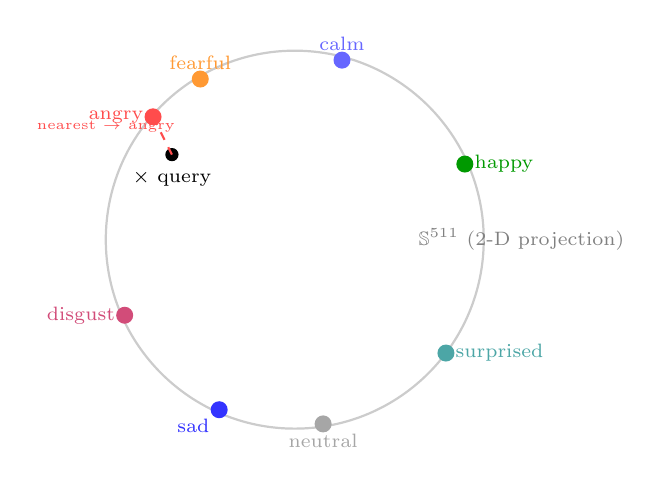
\begin{tikzpicture}[scale=1.2]
  % Unit circle
  \draw[gray!40,thick] (0,0) circle (2cm);
  \node[font=\scriptsize,gray] at (2.4,0) {$\mathbb{S}^{511}$ (2-D projection)};

  % 8 centroids
  \fill[red!70]    (-1.5, 1.3) circle (0.09) node[left,font=\scriptsize]{angry};
  \fill[blue!60]   (0.5, 1.9)  circle (0.09) node[above,font=\scriptsize]{calm};
  \fill[purple!70] (-1.8,-0.8) circle (0.09) node[left,font=\scriptsize]{disgust};
  \fill[orange!80] (-1.0, 1.7) circle (0.09) node[above,font=\scriptsize]{fearful};
  \fill[green!60!black] (1.8, 0.8)  circle (0.09) node[right,font=\scriptsize]{happy};
  \fill[gray!70]   (0.3,-1.95) circle (0.09) node[below,font=\scriptsize]{neutral};
  \fill[blue!80]   (-0.8,-1.8) circle (0.09) node[below left,font=\scriptsize]{sad};
  \fill[teal!70]   (1.6,-1.2)  circle (0.09) node[right,font=\scriptsize]{surprised};

  % Query point
  \fill[black] (-1.3, 0.9) circle (0.07);
  \node[font=\scriptsize,black] at (-1.3,0.65) {$\times$ query};

  % Nearest centroid line
  \draw[red!70,thick,dashed] (-1.3,0.9) -- (-1.5,1.3);
  \node[font=\tiny,red!70] at (-2.0,1.2) {nearest $\to$ angry};

\end{tikzpicture}
\caption{Conceptual 2-D projection of the 8 RAVDESS emotion centroids on
$\mathbb{S}^{511}$. A query embedding $\times$ is classified as the emotion
whose centroid it is closest to (highest dot product).}
\label{fig:centroid_geo}
\end{figure}

\begin{theorem}[Centroid Classifier Optimality Under Uniform Class Variance]
Let $\mathcal{E}_k$ be the set of projected embeddings for class $k$.
The centroid classifier $\hat{k} = \arg\max_k \mathbf{e} \cdot \mathbf{c}_k$
is the maximum-likelihood classifier under the assumption that each class
follows a von Mises-Fisher distribution on $\mathbb{S}^{511}$ with the
\emph{same} concentration parameter $\kappa$ for all classes.
When classes have unequal variances, it is a Bayes-optimal approximation
for equal prior probabilities $P(Y = k) = 1/8$.
\end{theorem}

\begin{proposition}[Why Centroid Classifier Over Neural Classifier?]
A centroid classifier:
\begin{enumerate}
  \item Requires \textbf{zero extra training} — uses the already-trained projection.
  \item Is \textbf{interpretable} — confidence = cosine distance to centroid.
  \item \textbf{Generalises well} with limited data (RAVDESS has $\approx$1,440 clips).
  \item Has \textbf{constant inference time} $O(K \cdot d) = O(8 \times 512)$
        regardless of corpus size.
\end{enumerate}
\end{proposition}

\begin{remark}[Plain-language]
Imagine 8 buckets, one per emotion.
During this offline step, you:
\begin{enumerate}
  \item Take every RAVDESS emotion clip, run it through AudioProjection,
        and drop the resulting 512-number vector into the matching bucket.
  \item Average all vectors in each bucket to find its ``centre of mass.''
  \item Rescale that centre so it lies exactly on the unit sphere.
  \item Save all 8 centres as an $8 \times 512$ matrix.
\end{enumerate}
At runtime, a new audio clip produces a single vector.
You ask: ``which of the 8 bucket-centres is this vector closest to?''
That is the emotion. No retraining needed.
\end{remark}

% ══════════════════════════════════════════════════
\section{Summary: Shared Embedding Space Properties}
% ══════════════════════════════════════════════════

\begin{table}[H]
\centering
\caption{Key mathematical properties of the shared embedding space}
\begin{tabularx}{\textwidth}{lXX}
\toprule
Property & Formula & Implication \\
\midrule
Unit-norm outputs & $\|\mathbf{e}\|_2 = 1$ & Cosine sim = dot product \\
Shared 512-d space & $\mathbf{e}_{\text{text}}, \mathbf{e}_{\text{audio}} \in \mathbb{S}^{511}$ & Cross-modal comparison \\
Frozen backbones & $\nabla_{\theta_{\text{BERT}}} = \nabla_{\theta_{\text{W2V}}} = \mathbf{0}$ & Only $\approx$987K params trained \\
Centroid classifier & $\hat{k} = \arg\max_k \mathbf{e} \cdot C_k$ & Zero extra training \\
Domain gate & $\sum_{t \in \mathcal{T}} \mathbf{1}[t \in s] \geq 2$ & Simple BoW switch \\
\bottomrule
\end{tabularx}
\end{table}

\begin{table}[H]
\centering
\caption{Free-tier technology stack of \texttt{encoders.py}}
\begin{tabular}{lll}
\toprule
Component & Tool & Cost \\
\midrule
STT & Whisper base (local, no API key) & Free \\
Audio features & Wav2Vec 2.0 (HuggingFace) & Free \\
Text features & BERT-base-uncased (HuggingFace) & Free \\
NER & spaCy \texttt{en\_core\_web\_sm} / \texttt{en\_core\_sci\_sm} & Free \\
LLM (downstream) & Groq API / Llama-3.1-8B & Free tier \\
\bottomrule
\end{tabular}
\end{table}

\begin{corollary}[Extensibility to New Modalities]
Adding a new modality (e.g., image via ResNet-50) requires only:
\begin{enumerate}
  \item A new projection head $f_\phi : \mathbb{R}^{d_{\text{new}}} \to \mathbb{S}^{511}$
        with L2-normalised output.
  \item A contrastive loss pairing the new modality with an existing one.
  \item A new concrete subclass of \texttt{BaseAudioEncoder} or \texttt{BaseTextEncoder}.
\end{enumerate}
No changes to the downstream retriever, KG, LLM, or TTS pipeline are required.
\end{corollary}

\end{document}
